\documentclass[full]{l3doc}
\usepackage[scheme=plain]{ctex}
\usepackage{enumitem}
\usepackage{indentfirst}
\usepackage{titling}
\usepackage{geometry}
\usepackage{fancyvrb-ex}
\usepackage{joinbox}

\IndexPrologue
  {
    \section*{Index}
    \markboth{Index}{Index}
    \addcontentsline{toc}{section}{Index}
    The~italic~numbers~denote~the~pages~where~the~
    corresponding~entry~is~described,~
    numbers~underlined~point~to~the~definition,~
    all~others~indicate~the~places~where~it~is~used.
  }

\newcommand\tikzmark[1]{\tikz \coordinate[overlay, remember picture] (#1);}

\geometry{
  left=4.5cm,
  right=2cm,
  top=2cm,
  bottom=2cm,
}
\hypersetup {
  CJKbookmarks,
  bookmarksopen,
  bookmarksopenlevel=3,
  pdfstartview=FitH,
  pdfinfo = {
   Title = The package joinbox ,
   Subject = A LaTeX3 package ,
   Author = Geng Nan
 }
}

\DoNotIndex{\begin, \end}
\setlength{\parskip}{\medskipamount}
\DeclareDocumentEnvironment { noteen } { +b } {
  \par\textbf{\textsf{NOTE:~}}#1\par
} {}
\DeclareDocumentEnvironment { notezh } { +b } {
  \par\textbf{\textsf{注意:~}}#1\par
} {}

\AtEndDocument{
  \newgeometry{
    left=2cm,
    right=2cm,
    top=2cm,
    bottom=2cm
  }
  \PrintIndex
}

\ExplSyntaxOn
\dim_new:N \l__my_syntax_dim
\box_new:N \g__my_syntax_box
\NewDocumentEnvironment { Syntax } { s }
  {
    \dim_set:Nn \l__my_syntax_dim
      { \textwidth }
    \hbox_gset:Nw \g__my_syntax_box
      \small \ttfamily
      \begin{minipage}[t]{\l__my_syntax_dim}
        \raggedright\obeyspaces\obeylines
  }
  {
      \end{minipage}
    \hbox_gset_end:
    \IfValueF { #1 } { \smallskip }
    \box_use_drop:N \g__my_syntax_box
    \smallskip
  }

\DeclareDocumentEnvironment { Description } { o +b } {
  \hbox_set:Nn \l_tmpa_box { #1 }
  \dim_set:Nn \l_tmpa_dim { \box_wd:N \l_tmpa_box }
  \begin{itemize}[labelwidth=\l_tmpa_dim, align=left]
    #2
  \end{itemize}
} {  }

\keys_define:nn { joinbox/doc } {
  opt  .tl_set:N = \l_opt_tl,
  desc .tl_set:N = \l_desc_tl,
  init .tl_set:N = \l_init_tl,
  init .initial:n = init-none,
}

\box_new:N \l__option_box
\NewDocumentEnvironment { option } { m +b } {
  \keys_set:nn { joinbox/doc } { #1 }
  \hbox_set:Nw \l__option_box
    \small \ttfamily
    \begin{minipage}[t]{\textwidth}
      \obeyspaces\obeylines
      \textcolor{red}{
        \l_opt_tl
        \exp_args:Nx\SpecialOptionIndex{\l_opt_tl}
      }
      {~}\l_desc_tl
      \hfill(
      \tl_if_eq:NnTF \l_init_tl { init-none } { no~value }
        { initially~\texttt{\l_init_tl} }
      )
    \end{minipage}
  \hbox_gset_end:
  \box_use_drop:N \l__option_box
  #2
  \medskip
} {  }

\DeclareDocumentCommand \opt { O{} m }
  { \__codedoc_cmd:no {#1} { #2 } }
\ExplSyntaxOff

\def\vers{\texttt{v1.0.3}
\thanks{\url{https://gitee.com/nwafu_nan/joinbox}}
}

\begin{document}
\title{
  \pkg{joinbox}盒子拼接宏包
  \rlap{\makebox[4cm][r]{
    \normalsize $\Longrightarrow$ \color{red}
    \protect\hyperlink{en}{English Version}
    \protect\hypertarget{zh}{}
  }}
}
\author{\textit{耿楠} \texttt{<nangeng@nwafu.edu.cn>}}
\date{\the\year 年\the\month 月\the\day 日\qquad \vers
}
\maketitle

{\small
\tableofcontents
}
\newpage

\begin{documentation}

\section{引言}

\pkg{joinbox}是一个基于\pkg{l3coffins}用\pkg{Expl3}开发的
盒子拼接宏包，它用于实现盒子的垂直或水平拼接。垂直拼接
会以各对象等宽的方式拼接，而水平拼接会以各对象等高的方式
拼接。

该宏包提供了\tn{joinbox}、\tn{joinboxes}和\tn{joinfigs}三个拼接
命令。其中，\tn{joinbox}用于拼接两个独立对象，\tn{joinboxes}用于
拼接一组对象，\tn{joinfigs}用于拼接多个图像。这三个命令的不带*(星号)
版本用于垂直拼接，而带*(星号)的版本用于水平拼接。

同时，该宏包还提供了\tn{joinset}命令用于对输出基线、尺寸和拼接间距进行设置。

\section{用户接口}

\subsection{\cs{joinbox}拼接两个对象命令}

\begin{function}{\joinbox,\joinbox*}
  \begin{syntax}
    \cs{joinbox} \oarg{拼接选项} \marg{对象1} \marg{对象2}
    \cs{joinbox*} \oarg{拼接选项} \marg{对象1} \marg{对象2}
  \end{syntax}

\end{function}

  用于拼接两个对象。 该命令需要用两个必选参数\marg{对象1}和
  \marg{对象2}指定需要拼接的对象。拼接对象将被置于coffin中，
  然后按需求进行拼接。

  \marg{对象1}或\marg{对象2}可以置空，但两者不能同时为空。

  在\oarg{拼接选项}中，可以通过逗号分隔的key-value指定输出结果
  基线位置、 输出尺寸(垂直拼接是输出宽度，水平拼接是输出高度)
  和拼接间距。

\subsection{\cs{joinboxes}拼接多个对象命令}

\begin{function}{\joinboxes,\joinboxes*}
  \begin{syntax}
    \cs{joinboxes} \oarg{拼接选项} \marg{拼接内容列表}
    \cs{joinboxes*} \oarg{拼接选项} \marg{拼接内容列表}
  \end{syntax}

\end{function}

  用于拼接多个对象。该命令需要用一个必选参数\marg{拼接内容列表}，
  指定需要拼接的内容，不同内容之间用英文逗号进行分隔，若内容中含
  有空格或逗号，则需要将其置于|{}|分组中。最少需要有1个拼接内容。

  在\oarg{拼接选项}中，可以通过逗号分隔的key-value指定结果基线位置、
  输出尺寸(垂直拼接是输出宽度，水平拼接是输出调试)、拼接间距。

\subsection{\cs{joinfigs}拼接多个图像命令}

\begin{function}{\joinfigs,\joinfigs*}
  \begin{syntax}
    \cs{joinfigs} \oarg{拼接选项} \marg{文件名称列表}
    \cs{joinfigs*} \oarg{拼接选项} \marg{文件名称列表}
  \end{syntax}

\end{function}

  用于拼接多个图像。该命令需要用一个必选参数\marg{文件名称列表}
  指定需要拼接图像，文件名称中可以包含路径，不同文件名称之间用
  英文逗号进行分隔。最少需要有1个图像文件名称。

  在\oarg{拼接选项}中，可以通过逗号分隔的key-value指定结果基线位置、
  输出尺寸(垂直拼接是输出宽度，水平拼接是输出调试)、拼接间距。

\subsection{\cs{joinset}}
\begin{function}{\joinset}
  \begin{syntax}
    \cs{joinset} \marg{拼接选项}
  \end{syntax}

\end{function}

  用于通过逗号分隔的key-value指定拼接结果中的基线位置、
  输出尺寸(垂直拼接是输出宽度，水平拼接是输出调试)、拼接间距。

\section{拼接选项}

\begin{option}{ opt = baseline, desc = {= \meta{t,vc,H,b}}, init=b }
  设置joinbox或joinfigs拼接结果的输出基线位置，目前支持：
\end{option}\\
\begin{Description}
  \item |t|--- 盒子顶端水平线、
  \item |vc|---盒子水平中心线、
  \item |H|---盒子内容基线、
  \item |b|---盒子底端水平线。
\end{Description}
\begin{notezh}
  可以省略\texttt{baseline}键名，但其值只能取|t|、|vc|、|H|和|b|。
\end{notezh}

\begin{SideBySideExample}[frame=single,numbers=left,xrightmargin=.45\linewidth,gobble=2]
  默认基线->\fbox{
    \joinbox{\LaTeX 科技排版}
            {\LaTeX~Typesetting}
  }

  指定基线->\fbox{
    \joinbox[baseline=t]{\LaTeX 科技排版}
                        {\LaTeX~Typesetting}
  }

  省略键名->\fbox{
    \joinbox[vc]{\LaTeX 科技排版}
                        {\LaTeX~Typesetting}
  }
\end{SideBySideExample}

\bigskip

\begin{option}{ opt = outlen, desc = {= \meta{dim}}, init=0pt }
  设置joinbox或joinfigs拼接结果的输出尺寸，对于垂直拼接，设置
  输出宽度，对于水平拼接，设置输出高度。

  若指定的输出尺寸$\le 0$，则表示使用被拼接对象中的最小尺寸输出。
\end{option}\\
\begin{notezh}
  可以省略\texttt{outlen}键名，但值只能取|dim|尺寸或尺寸表达式。

  当同时省略\texttt{baseline}键名和\texttt{outlen}键名时，如果
  键值为不支持的\texttt{baseline}，也是不|dim|尺寸或|dim|尺寸表达式，
  则会出错。
\end{notezh}
\begin{SideBySideExample}[frame=single,numbers=left,xrightmargin=.45\linewidth,gobble=2]
  输出宽度\fbox{
    \joinbox[outlen=2cm]{\LaTeX 科技排版}
                        {\LaTeX~Typesetting}
  }

  输出高度\fbox{
    \joinbox*[outlen=0.2cm]{\LaTeX 科技排版}
                        {\LaTeX~Typesetting}
  }

  省略键名\fbox{
    \joinbox[3cm]{\LaTeX 科技排版}
                        {\LaTeX~Typesetting}
  }
\end{SideBySideExample}

\bigskip

\begin{option}{ opt = sep, desc = {= \meta{dim}}, init=0pt }
  设置拼接对象之间的间距。
\end{option}\\
\begin{SideBySideExample}[frame=single,numbers=left,xrightmargin=.45\linewidth,gobble=2]
  垂直间距\fbox{
    \joinbox[sep=5pt]{\LaTeX 科技排版}
                  {\LaTeX~Typesetting}
  }

  水平间距\fbox{
    \joinbox*[outlen=0.2cm,sep=5pt]
             {\LaTeX 科技排版}
             {\LaTeX~Typesetting}
  }
\end{SideBySideExample}

\section{多盒子拼接}

可以使用\tn{joinboxes}命令一次拼接多个对象，不同对象间用逗号进行分隔，
如果对象包含逗号，则需要将该对象置于|{}|构成的分组中。

\begin{SideBySideExample}[frame=single,numbers=left,xrightmargin=.45\linewidth,gobble=2]
  \joinboxes[sep=2pt]{%
                      \LaTeX 科技排版,
                      {\LaTeX, Typesetting}
                     }

  \joinboxes*[0.2cm,sep=2pt]{%
                      \LaTeX 科技排版,
                      {\LaTeX, Typesetting}
                     }
\end{SideBySideExample}

\section{嵌套拼接}

可以嵌套使用\tn{joinbox}、\tn{joinboxes}命令以实现复杂对象拼接。

\begin{SideBySideExample}[frame=single,numbers=left,xrightmargin=.45\linewidth,gobble=2]
  \joinbox*[outlen=0.04\textheight,sep=-5pt]
        {
          \joinbox[sep=5pt]{\LaTeX 科技排版}
            {\qquad\LaTeX~Typesetting\qquad}
        }{
          
\includegraphics[scale=0.2]{expl3}
        }
\end{SideBySideExample}

\section{图像拼接}

\subsection{原始图像}

\begin{center}
  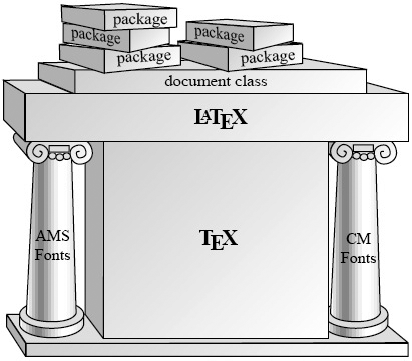
\includegraphics[scale=0.4]{latexframe}\quad
  
\includegraphics[scale=0.4]{tl-lion}\quad
  
\includegraphics[scale=0.4]{expl3}
\end{center}

\subsection{垂直拼接图像}

垂直拼接时，各对象保持相同宽度。

\begin{SideBySideExample}[frame=single,numbers=left,xrightmargin=.45\linewidth,gobble=2]
  \joinfigs[outlen=3cm, sep=5pt]
           {latexframe, tl-lion, expl3}
\end{SideBySideExample}

\subsection{水平拼接图像}

水平拼接时，各对象保持相同高度。

\begin{SideBySideExample}[frame=single,numbers=left,xrightmargin=.45\linewidth,gobble=2]
  \joinfigs*[outlen=1.3cm, sep=5pt]
           {latexframe, tl-lion, expl3}
\end{SideBySideExample}

\subsection{嵌套拼接图像}

可以嵌套使用\tn{joinbox}、\tn{joinboxes}或\tn{joinfigs}命令以实现复杂图像拼接。

\begin{SideBySideExample}[frame=single,numbers=left,xrightmargin=.45\linewidth,gobble=2]
  \joinbox*[0.20\textheight, sep=5pt]
          {
            \joinfigs[0.25\textwidth]
              {latexframe, tl-lion, expl3}
          }{
            \joinfigs[0.25\textwidth]
              {expl3, tl-lion, latexframe}
          }
\end{SideBySideExample}

\begin{SideBySideExample}[frame=single,numbers=left,xrightmargin=.45\linewidth,gobble=2]

  \joinboxes*[0.15\textheight, sep=5pt]{%
          {
            \joinfigs[0.25\textwidth]
              {latexframe, tl-lion, expl3}
          },
          {
            \joinfigs[0.25\textwidth]
              {tl-lion, latexframe,expl3}
          },
          {
            \joinfigs[0.25\textwidth]
              {expl3, tl-lion, latexframe}
          }
      }
\end{SideBySideExample}

\section{单对象拼接}

\tn{joinbox}、\tn{joinboxes}或\tn{joinfigs}命令也可以实现只``伪拼接''
一个对象，此时，则可以通过选项调整输出的基线位置和大小。

\begin{SideBySideExample}[frame=single,numbers=left,xrightmargin=.45\linewidth,gobble=2]
  \joinbox{\LaTeX 科技排版}{}

  \joinbox[4cm]{}{\LaTeX 科技排版}

  \joinboxes{\LaTeX 科技排版}
\end{SideBySideExample}

\begin{SideBySideExample}[frame=single,numbers=left,xrightmargin=.45\linewidth,gobble=2]
  基线位置->\joinfigs[vc,4cm]{latexframe}
\end{SideBySideExample}

\section{垂直盒子拼接}

由于是基于Expl3的\tn{hcoffin_set:Nn}函数构造内部盒子实现拼接的，因此，
待拼接内容中的|\\|和\tn{par}(包括空行)等断行和分段命令将失效。此时，
可以先用\tn{parbox}等命令或\env{minipage}等环境先构建一个垂直盒子，
然后再将构造的垂直盒子作为一个对象进行拼接。

\begin{SideBySideExample}[frame=single,numbers=left,xrightmargin=.45\linewidth,gobble=2]
  \joinbox{
    \parbox{8em}{
      \centering
      \LaTeX 科技排版

      \LaTeX~Typesetting
    }
  }{
\includegraphics{expl3}}
\end{SideBySideExample}

\begin{SideBySideExample}[frame=single,numbers=left,xrightmargin=.45\linewidth,gobble=2]
  \joinboxes*{
    {
      \begin{minipage}{8em}
        \centering
        \LaTeX 科技排版

        \LaTeX~Typesetting
      \end{minipage}
    },
    {
\includegraphics{expl3}}
  }
\end{SideBySideExample}

\title{
  \pkg{joinbox} package for Joinning Boxs or Figures
  \rlap{\makebox[2.5cm][r]{
    \normalsize $\Longrightarrow$ \color{red}
    \protect\hyperlink{zh}{中文版本}
    \protect\hypertarget{en}{}
  }}
}
\author{Nan Geng \texttt{<nangeng@nwafu.edu.cn>}}
\date{\today\qquad \vers}
\maketitle

\section{Introduction}

\pkg{joinbox} is a box joinning package based on l3coffins developed with Expl3,
which provides the \cs{joinbox}, \cs{joinboxes} and \cs{joinfigs} macros for
vertical or horizontal joinning of boxes. The typout baseline, size and seperated
space can be set up with the options or \cs{joinset} macro.

Boxes can be joined vertically or horizontally. When using vertical joinning, all
boxes to be joined will keep same width, while when using horizontal joined, all
boxes to be joined will keep same height.

The \cs{joinbox}, \cs{joinboxes} and \cs{joinfigs} macros without star are used
for vertical joinning, while the \cs{joinbox*}, \cs{joinboxes*} and
\cs{joinfigs*} with star are used for horizontal joinning.

\section{Interfaces}

\subsection{\cs{joinbox} for Two Contents Joinning }

\begin{function}{\joinbox,\joinbox*}
  \begin{syntax}
    \cs{joinbox} \oarg{options} \marg{content1} \marg{content2}
    \cs{joinbox*} \oarg{options} \marg{content1} \marg{content2}
  \end{syntax}

\end{function}

  Used to join two contents. It requires two arguments \marg{content1} and
  \marg{content2} to specify the objects to be joined. The contents will
  be placed in the coffin respectively and then joined.

  \marg{content1} or \marg{content2} can be null, but both cannot be null at
  the same time.

  In the \oarg{options}, the typeout baseline, typeout size
  (vertical joinning is width, horizontal joinning is height), and 
  joinning seperate spacing can be specified with \textit{key-value}.

\subsection{\cs{joinboxes} for Content Sets Joinning}

\begin{function}{\joinboxes,\joinboxes*}
  \begin{syntax}
    \cs{joinboxes} \oarg{options} \marg{content list}
    \cs{joinboxes*} \oarg{options} \marg{content list}
  \end{syntax}

\end{function}

  Used for joinning multiple contents. This command requires a
  argument\marg{content list} to specify the content to be joined.
  They should be separated by commas, it should. Items which contain
  either spaces or commas should be surrounded by braces.
  At least one content is required.

  In the \oarg{options}, the typeout baseline, typeout size
  (vertical joinning is width, horizontal joinning is height), and
  joinning seperate spacing can be specified with \textit{key-value}.

\subsection{\cs{joinfigs} for Figure Sets Joinning}

\begin{function}{\joinfigs,\joinfigs*}
  \begin{syntax}
    \cs{joinfigs} \oarg{options} \marg{namelist}
    \cs{joinfigs*} \oarg{options} \marg{namelist}
  \end{syntax}

\end{function}

  Used for joinning multiple images. This command requires a argument\marg{namelist}
  to specify the image to be joined. The file name can include a path, 
  and different file names should be separated by commas. 
  At least one image file name is required.

  In the \oarg{options}, the typeout baseline, typeout size
  (vertical joinning is width, horizontal joinning is height), and 
  joinning seperate spacing can be specified with \textit{key-value}.

\subsection{\cs{joinset} for Settings}
\begin{function}{\joinset}
  \begin{syntax}
    \cs{joinset} \marg{options}
  \end{syntax}

\end{function}

  Used to set the typeout baseline, typeout size
  (vertical joinning is width, horizontal joinning is height), and 
  joinning seperate spacing with \textit{key-value}.

\section{Options}

\begin{option}{ opt = baseline, desc = {= \meta{t,vc,H,b}}, init=b }
  Set typeout baseline, currently as follows:
\end{option}\\
\begin{Description}
  \item |t|--- a pole running along the top edge of the bounding box of the coffin;
  \item |vc|---a pole running horizontally through the centre of the coffin half-way between the
bottom and top edges of the bounding box (i.e. the “vertical centre”);
  \item |H|---a pole running along the baseline of the typeset material contained in the coffin;
  \item |b|---a pole running along the bottom edge of the bounding box of the coffin.
\end{Description}
\begin{noteen}
  In most cases, you can omit the baseline key names and write only it's value. 
  But the value must be t, vc, H or b.
\end{noteen}

\begin{SideBySideExample}[frame=single,numbers=left,xrightmargin=.45\linewidth,gobble=2]
  default->\fbox{
    \joinbox{Hello \LaTeX}
            {\LaTeX~Typesetting}
  }

  top->\fbox{
    \joinbox[baseline=t]{Hello \LaTeX}
                        {\LaTeX~Typesetting}
  }

  omit baseline->\fbox{
    \joinbox[vc]{Hello \LaTeX}
                        {\LaTeX~Typesetting}
  }
\end{SideBySideExample}

\bigskip

\begin{option}{ opt = outlen, desc = {= \meta{dim}}, init=0pt }
  Used to set typeout size, vertical joinning is width and horizontal joinning is height.

  If $outlen\le 0$，then the typeout size is minimal size of all contents.
\end{option}\\
\begin{noteen}
  In most cases, you can omit the outlen key names and write only it's value. 
  But the value must be dimension expression.

  When omitting both the |baseline| key name and the |outlen| key name,
  an error occurs if the key value is an unsupported |baseline| and
  not |dim| or |dim| expression.
\end{noteen}

\begin{SideBySideExample}[frame=single,numbers=left,xrightmargin=.45\linewidth,gobble=2]
  width: \fbox{
    \joinbox[outlen=2cm]{Hello \LaTeX}
                        {\LaTeX~Typesetting}
  }

  height: \fbox{
    \joinbox*[outlen=0.2cm]{Hello \LaTeX}
                        {\LaTeX~Typesetting}
  }

  omit outlen: \fbox{
    \joinbox[2cm]{Hello \LaTeX}
                 {\LaTeX~Typesetting}
  }
\end{SideBySideExample}

\bigskip

\begin{option}{ opt = sep, desc = {= \meta{dim}}, init=0pt }
  Used to set joinning seperate spacing.
\end{option}\\
\begin{SideBySideExample}[frame=single,numbers=left,xrightmargin=.45\linewidth,gobble=2]
  vertical sep: \fbox{
    \joinbox[sep=5pt]{Hello \LaTeX}
                  {\LaTeX~Typesetting}
  }

  horizontal sep: \fbox{
    \joinbox*[outlen=0.2cm,sep=5pt]
             {Hello \LaTeX}
             {\LaTeX~Typesetting}
  }
\end{SideBySideExample}

\section{Multiple Joinning}

The \tn{joinboxes} can join multiple contents.

\begin{SideBySideExample}[frame=single,numbers=left,xrightmargin=.45\linewidth,gobble=2]
  \joinboxes[sep=2pt]{%
                      {Hello, \LaTeX},
                      \LaTeX~Typesetting
                     }

  \joinboxes*[0.2cm,sep=2pt]{%
                      {Hello, \LaTeX},
                      \LaTeX~Typesetting
                     }
\end{SideBySideExample}

\section{Nested Joinning}

The \tn{joinbox} \tn{joinboxes} can be nested to get complex joinning.

\begin{SideBySideExample}[frame=single,numbers=left,xrightmargin=.45\linewidth,gobble=2]
  \joinbox*[outlen=0.04\textheight,sep=-5pt]
        {
          \joinbox[sep=5pt]{Hello \LaTeX}
            {\qquad\LaTeX~Typesetting\qquad}
        }{
          
\includegraphics[scale=0.2]{expl3}
        }
\end{SideBySideExample}

\section{Figures Joinning}

\subsection{Original}

\begin{center}
  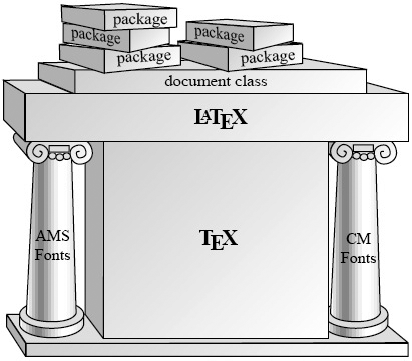
\includegraphics[scale=0.4]{latexframe}\quad
  
\includegraphics[scale=0.4]{tl-lion}\quad
  
\includegraphics[scale=0.4]{expl3}
\end{center}

\subsection{Vertical Joinning}

When using vertical joinning, all boxes to be joined will keep same width.

\begin{SideBySideExample}[frame=single,numbers=left,xrightmargin=.45\linewidth,gobble=2]
  \joinfigs[outlen=3cm, sep=5pt]
           {latexframe, tl-lion, expl3}
\end{SideBySideExample}

\subsection{Horizontal Joinning}

When using horizontal joined, all boxes to be joined will keep same height.

\begin{SideBySideExample}[frame=single,numbers=left,xrightmargin=.45\linewidth,gobble=2]
  \joinfigs*[outlen=1.3cm, sep=5pt]
           {latexframe, tl-lion, expl3}
\end{SideBySideExample}

\subsection{Nested Joinning}

The\tn{joinbox}, \tn{joinboxes}, or \tn{joinfigs} macros
can be nested for complex image joinning.

\begin{SideBySideExample}[frame=single,numbers=left,xrightmargin=.45\linewidth,gobble=2]
  \joinbox*[0.20\textheight, sep=5pt]
          {
            \joinfigs[0.25\textwidth]
              {latexframe, tl-lion, expl3}
          }{
            \joinfigs[0.25\textwidth]
              {expl3, tl-lion, latexframe}
          }
\end{SideBySideExample}

\begin{SideBySideExample}[frame=single,numbers=left,xrightmargin=.45\linewidth,gobble=2]
  \joinboxes*[0.15\textheight, sep=5pt]{%
          {
            \joinfigs[0.25\textwidth]
              {latexframe, tl-lion, expl3}
          },
          {
            \joinfigs[0.25\textwidth]
              {tl-lion, latexframe,expl3}
          },
          {
            \joinfigs[0.25\textwidth]
              {expl3, tl-lion, latexframe}
          }
      }
\end{SideBySideExample}

\section{Single Joinning}

The \tn{joinbox}, \tn{joinboxes}, or \tn{joinfigs} macros can also be
used to ``pseudo-joinning'' only one object, in which case the baseline
and size of the output can be adjusted with the options.

\begin{SideBySideExample}[frame=single,numbers=left,xrightmargin=.45\linewidth,gobble=2]
  \joinbox{Hello \LaTeX}{}

  \joinbox[4cm]{}{Hello \LaTeX}

  \joinboxes{Hello \LaTeX}
\end{SideBySideExample}

\begin{SideBySideExample}[frame=single,numbers=left,xrightmargin=.45\linewidth,gobble=2]
  baseline->\joinfigs[vc,4cm]{latexframe}
\end{SideBySideExample}

\section{Vertical Box Joinning}

Since joinbox is realized by constructing two internal boxes based on
the \tn{hcoffin_set:Nn} Expl3 function, line breaking and new paragraph
macros such as |\\| and \tn{par}(including blank lines) in the content
to be joined will be invalid. In this case, you can first construct a
vertical box using commands such as \tn{parbox} or environments such as
|minipage|, and then join the constructed vertical box as an object.

\begin{SideBySideExample}[frame=single,numbers=left,xrightmargin=.45\linewidth,gobble=2]
  \joinbox{
    \parbox{8em}{
      \centering
      Hello \LaTeX

      \LaTeX~Typesetting
    }
  }{
\includegraphics{expl3}}
\end{SideBySideExample}

\begin{SideBySideExample}[frame=single,numbers=left,xrightmargin=.45\linewidth,gobble=2]
  \joinboxes*{
    {
      \begin{minipage}{8em}
        \centering
        Hello \LaTeX

        \LaTeX~Typesetting
      \end{minipage}
    },
    {
\includegraphics{expl3}}
  }
\end{SideBySideExample}

\end{documentation}

\end{document}
